\section*{Sanctions as a Network Process \& the Importance of Reciprocity}
\label{neteffects}

A contribution of our study is to demonstrate why sanctions processes should be considered in a network context. To do so, we provide an example. Figure \ref{fig:spaghetti} presents the entire sanction-year network for the year 1984.  Nodes represent states and the directed edges denote senders and receivers of sanctions. The nodes are colored by the geographic position of a country, for example, countries in North America are colored in shades of red, and Asia in shades of yellow to green. This figure is complex, showing that each yearly network contains important information about state behavior, whereby numerous states are involved in multiple sanction cases during this individual year. IR scholars typically treat each dyad as independent, despite that a singular actor, such as the USA, likely exist within multiple dyads. The appearance of multiple actors in multiple rows of the data violates assumptions of independence. Theoretically, however, this also means that scholars are unable to include second-order dependencies such as reciprocity into their analyses. While studies of international relations tend to recognize the interdependent nature of state behavior in the theoretical sense, they often fail to uphold this theoretical intuition in empirical analysis. Early attempts are noteworthy \citep{goldstein1991reciprocity, keohane1989reciprocity} and more recent work has continued to address this concern \citep{cranmer2014reciprocity, mitchell2001} yet studies on sanction compliance have not incorporated these insights. 

\begin{figure}[ht]
  \centering
  \begin{tabular}{c}
	  \includegraphics[width=1\textwidth]{84net-crop} \\
	  \includegraphics[width=0.45\textwidth]{MapLegend}
  \end{tabular}
  \caption{Here we show the sanction network in 1984, nodes are colored by geographic coordinates of countries. Data for sanction cases comes from \citet{morgan2009threat}.}
  \label{fig:spaghetti}
\end{figure}
\FloatBarrier


\begin{center}
\textit{Theoretical Expectations of Reciprocity and State Behavior}\\
\end{center}

Assuming that sanctions processes are best considered through a network lens, we can then move forward to better incorporate the concept of reciprocity into our analysis. Given the wide range of literature on reciprocity in the study of international relations and foreign policy, we argue that it is necessary to consider how reciprocity plays a role in determining why, and when, sanctions end.

In studies of social and economic behavior, direct reciprocity--the notion that actors learn to ``respond in kind" to one another--is argued to be an essential component of behavior.\footnote{For example, see \cite{bolton:1998, charness:2002, charness:2004, cox:2007, cox:2004}.} The idea that individuals, or collectives, observe previously cooperative (or conflictual) behavior from others, and include this information into their own decision-making process, is a concept given great value for determining strategic outcomes. For example, reciprocity is shown to influence interactions across diverse settings including tax compliance \citep{smith:1990}, wage selection \citep{campbell:1997}, and strike breaking \citep{brett:1998}. Reciprocity is also shown to play a critical role in the development of interethnic attitudes whereby groups tend to reflect the attitudes that other groups hold toward them \citep{berry:1979}. 

Intuition about reciprocity's effect on the behavior of individuals also extends to aggregate analysis. International relations and foreign policy scholars have expressed a long standing interest in how reciprocity influences the evolution of cooperative and conflictual interactions among states \citep{keohane1989reciprocity, richardson1960}. \cite{rajmaira:1990} argue that reciprocity determines long-term foreign policy behavior among superpowers via norms creation. The authors importantly point out that reciprocity is a dynamic mechanism that changes over time. They show that while mutual reactivity between superpowers is often weak, high peaks in reciprocity create long-lasting and influential norms of behavior between countries. In other realms of international politics, reciprocity plays a key role in formulating expectations of state behavior. \cite{ward1981} even argued that reciprocity is a ``golden rule" of politics between nations.  Osiel similarly notes, ``It is an empirical datum that people tend to respond to others with an implicit policy of like for like and that this facilitates cooperation between them. This elementary fact has profound implications for the effective design of law and institutions.'' \cite[p. 19]{osiel:2009}. Reciprocity has long been recognized by IR scholars as an important mechanism for the enforcement of agreements and instantiation of cooperation. 

While reciprocity receives little attention in sanctions research, the literature instead focuses on how specific types of relationships between senders and targets--such as alliances and trade ties--expedite sanction resolution. The core mechanisms driving sanction outcomes are thus characterized in terms of a cost-benefit analysis, ignoring the plausible role that reciprocity plays in driving state behavior. Underlying the relational dimensions noted in the literature is the implicit argument that there are some set of countries from whom the sending of sanctions are more consequential, and will thus be complied to more quickly, than others. Much of this logic can be captured by the concept of reciprocity, yet by failing to directly consider reciprocity extant analyses ignores the rich history of interactions between countries. 

To establish the existence of reciprocity we assume that (1) reciprocity is best conceptualized as a long-term mechanism that develops a common expectation of behavior between states; (2) departures from established expectations of behavior are possible \citep{moore1995}; and (3) reciprocity is a necessary but not sufficient condition for influencing strategic behavior between states \citep{goldstein2001}. To the first point, early considerations of reciprocity characterized it as a reactive, short-term process (for example, tit for tat ``reactionary'' responses). Based on the evidence from \citet{rajmaira:1990} and others, we assume that reciprocity is a long-term process, born out by multiple interactions between actors over time. In this way, reciprocity becomes a norm of behavior, or a set of expectations about how actors engage with one another, over time.\footnote{The temporal effects of reciprocity are empirically demonstrated in literature focused both on super power behavior \citep{rajmaira:1990} and behavior in regional conflicts \citep{goldstein1997}.} Our second and third assumptions relate to one another in that we acknowledge other influences might effect state behavior and that at different periods states could have incentives to break away from established norms of behavior; this is important because it suggests that state behavior is not easily locked into unidirectional spirals \citep{moore1995}.

Reciprocity captures the development of strategic expectations that shape state's compliance behavior during sanctions. Overtime, previous reciprocal interactions inform a target state's decision to comply. Our basic intuition is that when a target state has a richer history of reciprocal compliance with sender states, they will more swiftly comply with the senders' demands. This intuition generates the primary hypothesis of this study, that \textit{reciprocity creates an underlying level of expected behavior which influences patterns of compliance among target states.} Importantly, our claim does not demand that reciprocity always work in some inherently ``good'' or ``bad'' way, but instead can prolong or shorten sanctions depending on which kind of past reciprocal behavior has occurred. This concept thus requires that we specify which forms of reciprocity should matter in the case of sanctions. We argue that reciprocity influences sanction outcomes through two forms: \textit{compliance reciprocity} and \textit{sanction reciprocity}. 

Compliance reciprocity represents a target states' cumulative history of compliance with a particular sender relative to all others in the network. We consider this relative history of compliance to indicate an established norm of cooperation between states. Thus, compliance reciprocity allows us to account for whether those who have a history of cooperative behavior with each other also tend to have more cooperative behavior in the future. In the sanction-duration context, states who receive sanctions from those with whom they have a history of reciprocal compliance are likely to comply sooner than they would with states to whom they have not had positive reciprocal interactions. Notably, this concept is distinct from a simple consideration of past instances of compliance with another state. Such a measure would completely ignore the fact that each state's actions are related to all other interactions between states. For example, if state $i$ complies often to state $j$, is state $i$ also more likely to comply with all other partner states? Or, relative to all other interactions, does state $i$ comply more frequently and uniquely with state $j$? The latter idea is the one explicated within our  concept of compliance reciprocity. Thus, reciprocity tells us information about the behavior between country $i$ and $j$ over time, relative to how country $i$ interacts with all other partners over time. 

We extend this intuition to our second key concept, \textit{sanction reciprocity}. Following the same idea as compliance reciprocity, sanction reciprocity considers how often a target state has received sanctions from the senders of any given sanction case relative to all other sanction interactions. The intuition behind this concept is that sanction reciprocity indicates a deepening resolve between states. The basic insight is that states whom continually respond to sanctions by sending sanctions of their own are signaling more conflictual rather than cooperative behavior over time. These strategic expectations are a dominating factor for the initiation of sanction compliance. 

\section*{Measuring Reciprocity}

To operationalize our measure of reciprocity, we turn to the Social Relations Model developed by \citet{kenny1994interpersonal} and \citet{dorff2013}. To illustrate, consider the matrix $X_{ij}$ below, in which we have six actors in a round robin (dyadic) format. These data are represented by the matrix below, which has a value for each of the thirty interactions, with the main diagonal remaining empty:

\singlespacing
\[
\left[
\begin{array}{cccccc}
 & X_{1}  & X_{2}  & X_{3} & X_{4} & X_{5} \\
X_{6}  &  & X_{7}  & X_{8} & X_{9} & X_{10} \\
X_{11}  & X_{12}  &    & X_{13} & X_{14} & X_{15} \\
X_{16}  & X_{17}  & X_{18}  &  & X_{19} & X_{20} \\
X_{21}  & X_{22}  & X_{23}  & X_{24} &   & X_{25} \\
X_{26}  & X_{27}  & X_{28}  & X_{29} & X_{30} &   \\
\end{array}
\right]
\]

\doublespacing
First, we begin with calculating the row column and total sums:

\begin{itemize}
	\item The totals for each \emph{ row} are denoted $X_{i \cdot}$ where $i$ is the row number, i.e.,
	~\\
	$X_{i \cdot} = \sum_{j=1}^{J} X_{ij}$;
	\item For each column the totals are denoted
	 $X_{\cdot i}$ where $i$ is the \emph{column} number; and 
	 \item The total over all rows and columns is given by $X_{\cdot \cdot} = \sum_i \sum_j X_{i,j}$.
 \end{itemize}
 
Given these quantities, one can calculate individual effects for a variety of concepts, such as the actor, partner, and unique dyadic effects, (as well as the variances attributed to each of these effects). The unique dyadic effects, or the reciprocal interactions between two countries within one pair, are calculated accounting for the general behavior of each country within the pair. Or, in other words, this measure captures the likelihood of $i$ complying to $j$ while controlling for the tendency of $i$ to comply to others and for $j$ to have had its sanctions complied to from other countries. By calculating the likelihood of a pair of countries complying to each other relative to how likely they are to comply to any other country we are able to control for nodal specific effects that often arise in networks. Specifically, we are able to account for the fact that some countries might simply be more likely to comply or refuse to comply to a sanction than others. Accounting for reciprocity in this way enables us to better measure the concept of reciprocity. 

 \begin{itemize}
	 \item []The actor effect for observation $i$ is the total of $i$'s row mean and column mean, minus the overall mean.  The means are just the sums, corrected for degrees of freedom, yielding an average row effect:\\
	\begin{equation}
	{\hat{a}_i = \frac{(n-1)^2}{n(n-2)} X_{i \cdot} + \frac{(n-1)}{n(n-2)} X_{\cdot i} -  \frac{n-1}{n-2} X_{\cdot \cdot} }
	\end{equation}
	\item[] Similarly the column mean for actor $i$ is \\
	\begin{equation}
	 \hat{b}_i = \frac{(n-1)^2}{n(n-2)} X_{\cdot i} + \frac{(n-1)}{n(n-2)} X_{i \cdot } -  \frac{n-1}{n-2} X_{\cdot \cdot}.\\
	 \end{equation}
	  For a symmetric matrix, the row effect and the column effect will be identical.
	\item[] The unique dyadic effect, or reciprocity for specific dyad $ij$, simply subtracts the row and column effects along with the overall mean out of the value for dyad $ij$. \\
	\begin{equation}
	\hat{g}_{ij} = X_{ij} - \hat{a}_i - \hat{b}_j - X_{\cdot \cdot}
	\end{equation}
 \end{itemize}

\doublespacing
The first two equations show how the final equation for reciprocity is calculated relative to the general actor and partner effects (or actor and partner average behavior) for each country.\footnote{\cite{kenny1994interpersonal} would suggest including the full compliment of the SRM into our model. We originally explored this approach, but gained little empirical leverage from it, and thus focus instead on the concept of reciprocity.} In figure \ref{fig:recipNet}, we provide a visualization of the \textit{compliance reciprocity} measure generated using the approach laid out above for 1972, 1992, and 2012. In each panel, we include the reciprocity scores for the ten countries that were most active in the sanctioning network at that year. Each of the edges are directional and indicate how likely a country is to reciprocate compliance from another; reciprocity scores that are negative are designated in red and positive are in blue. For example, in every panel shown here, Israel exclusively has negative incoming edges, indicating that the countries shown in these panels are all unlikely to reciprocate a compliant action from Israel. The implication of this is that even when Israel complies to an economic sanction from another state, that other state is relatively unlikely to comply to any sanctions sent by Israel. On the other hand, across all panels the United States almost exclusively has positive incoming edges, indicating that countries are very likely to reciprocate compliance behavior from the United States.  More interesting, however, is the fact that there exists significant variation in whether countries reciprocate behavior. Canada is likely to reciprocate the actions of the United Kingdom but not Russia or Japan, while others countries like France are likely to reciprocate the behavior of Japan but not others like Germany.

\begin{figure}[ht]
	\centering
	\caption{Reciprocity plots}
	\begin{tabular}{ccc}

	\subfloat[sub1][Compliance: 1972]{
		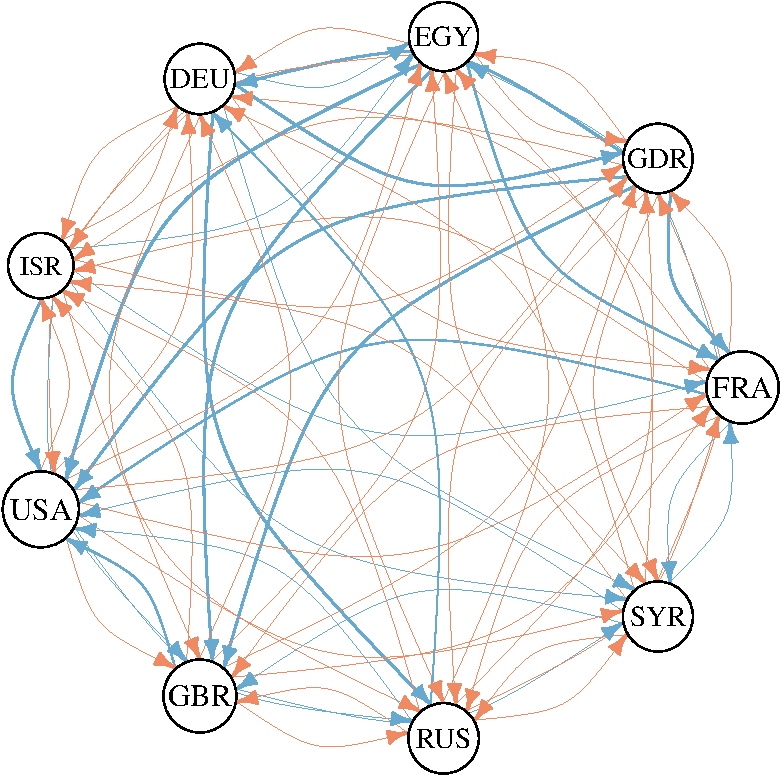
\includegraphics[width=.5\textwidth]{compNet_1972}
		\label{fig:comp72}} & 

	\subfloat[sub1][Compliance: 1992]{
		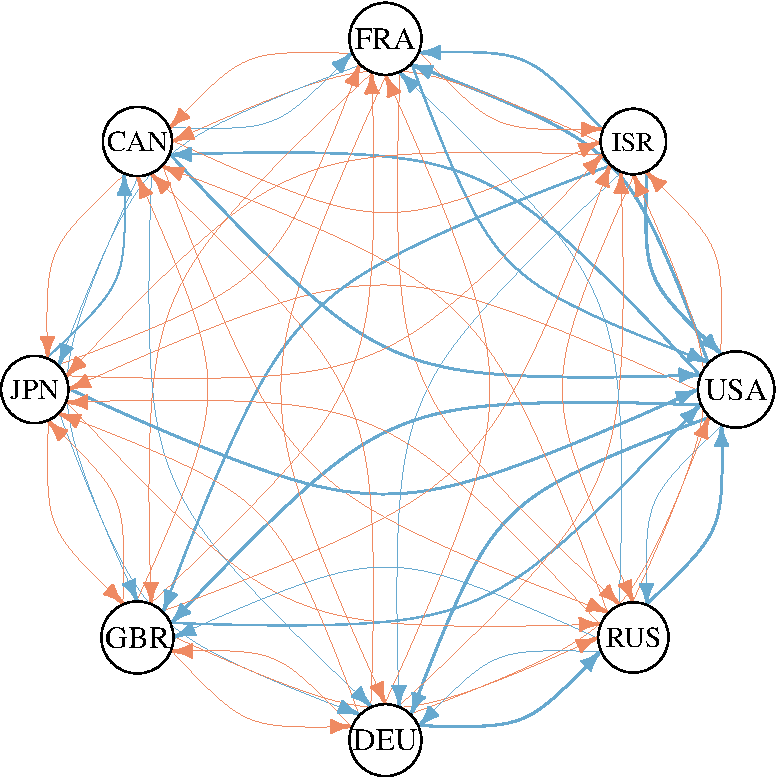
\includegraphics[width=.5\textwidth]{compNet_1992}
		\label{fig:comp92}} \\

	\multicolumn{2}{c}{\subfloat[sub1][Compliance: 2012]{
			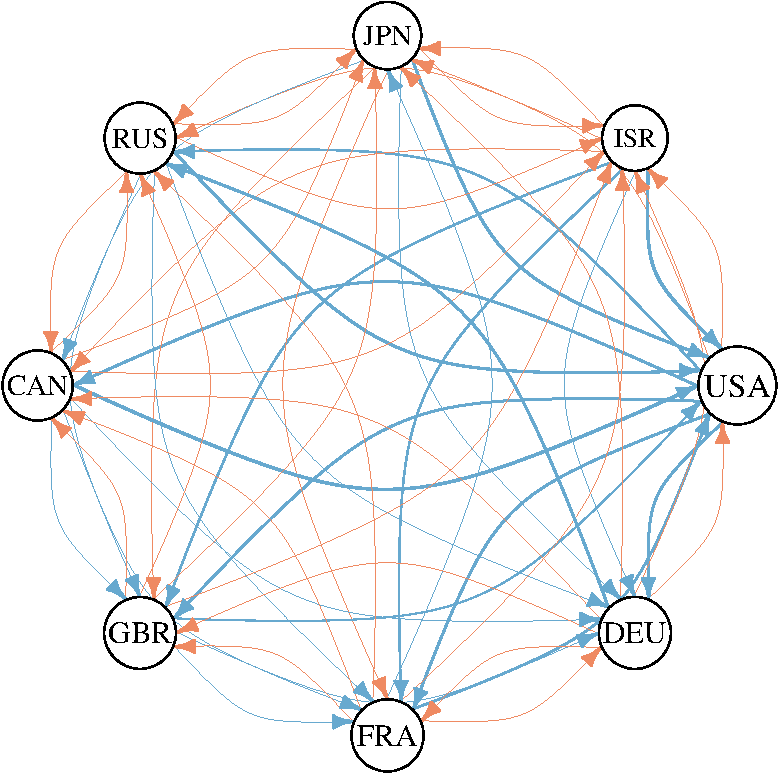
\includegraphics[width=.5\textwidth]{compNet_2012}
			\label{fig:comp02}}}


	\end{tabular}
	\label{fig:recipNet}
\end{figure}
\FloatBarrier